\chapter{روش‌های مبتنی بر یادگیری تقویتی}

کارهای تحقیقاتی در زمینه ی یادگیری تقویتی 
\LTRfootnote{reinforcement learning}
و پردازش زبان طبیعی در سال‌های اخیر رشد کرده است. در یادگیری تقویتی  یک عامل با محیط تعامل می‌کند و با آزمون و خطا، خط مشی بهینه را برای تصمیم گیری متوالی برای به حداکثر رساندن پاداش تجمعی آینده می‌آموزد. این پاداش می‌تواند یک معیار تعریف شده توسط توسعه دهنده بر اساس کار در حال حل باشد. در خلاصه‌سازی خودکار انتزاعی متن، نمونه‌هایی از چنین پاداش‌هایی ممکن است شامل حفظ برجستگی، مستلزم منطقی هدایت‌شده، و غیر افزونگی باشد. به طور کلی،  یادگیری تقویتی  در چهار حوزه مختلف برای بهبود خلاصه‌سازی خودکار استفاده می‌شود:

\section{یادگیری تقویتی برای حل مسائل عمیق توالی به دنباله}

استفاده از یادگیری تقویتی به منظور حل مسائل گوناگونی که مدل‌های دنباله به دنباله عمیق قادر به حل آن‌ها نیستند، امکانات بیشتری را فراهم می‌کند. به عنوان مثال، مشکلاتی مانند کمبود نوآوری در ایجاد خلاصه‌های خلاقانه و آموزنده و کاهش کیفیت خلاصه‌ها در صورت افزایش طول مقالات منبع، با استفاده از سیستم‌های یادگیری تقویتی و یادگیری خط‌مشی		\LTRfootnote{ policy learning} بهبود یافته است.
 علاوه بر این  مدل‌های دنباله به دنباله عمیق را نمی‌توان برای خلاصه کردن طیف گسترده ای از اسناد استفاده کرد، زیرا مدلی که بر روی یک مجموعه داده آموزش داده می‌شود، در یک مجموعه داده دیگر به خوبی عمل نمی‌کند و قابلیت تعمیم ندارد. رویکردهای مبتنی بر یادگیری تقویتی می‌تواند این  مشکل را با استفاده ازگرادیان خط مشی انتقادی
 \LTRfootnote{self-critic policy gradient}
  و ترکیب آن با یادگیری انتقالی
\LTRfootnote{Transfer Learning (TL) }
برای انتقال دانش از یک مجموعه داده به مجموعه دیگر برطرف کنند
\cite{DeepTL_RL}.

فریم‌ورک پوبرل
\LTRfootnote{PoBRL}
(ترکیب سیاست‌ها با حداکثر ارتباط حاشیه‌ای و یادگیری تقویتی) اهمیت، ارتباط و طول خلاصه را در زمینه خلاصه‌سازی چند سندی با جدا کردن مسئله بهینه‌سازی چند هدفه به مسائل فرعی کوچک‌تر که با استفاده از یادگیری تقویتی قابل حل هستند، بهینه می‌کند. 
اهمیت، ارتباط و طول خلاصه را در زمینه خلاصه‌سازی چند سندی با جدا کردن مسئله بهینه‌سازی چند هدفه به مسائل فرعی کوچک‌تر که قابل حل هستند، بهینه می‌کند.
این فریم‌ورک از الگوریتم حداکثر ارتباط حاشیه ای 
\LTRfootnote{ Maximal Marginal Relevance (MMR)}
برای استخراج اطلاعات مهم از اسناد استفاده می‌کند. استفاده از این الگوریتم باعث افزایش ارتباط بین  جملات و کاهش افزونگی می‌شود.
در ادامه با از یادگیری تقویتی رای بهینه سازی هر هدف به صورت جداگانه استفاده می کند و خط مشی های جداگانه ای را برای اهمیت، ارتباط و طول می آموزد
\cite{PoBRL}.
خلاصه‌سازی چند سندی شامل سر و کار داشتن با اطلاعات پیچیده و همپوشانی از منابع متعدد است. الگوریتم‌های یادگیری تقویتی می‌توانند با مدل‌سازی خلاصه‌سازی به عنوان یک فرآیند تصمیم‌گیری متوالی  پیچیدگی را مدیریت کنند و یاد بگیرند جملات مرتبط حاوی اطلاعات را برای خلاصه انتخاب کنند. علاوه بر این  یادگیری تقویتی امکان بهینه‌سازی همزمان اهداف متعدد مانند اهمیت، افزونگی و طول را فراهم می‌کند و موجب برقراری تعادل بین اهداف و تولید خلاصه‌‌های مختصر، مرتبط و غیر تکراری شوند.

%در مرحله بعد، چارچوب از یادگیری تقویتی برای بهینه سازی هر هدف به صورت جداگانه استفاده می کند. خط مشی های جداگانه ای را برای اهمیت، ارتباط و طول می آموزد.
%چارچوب مبتنی بر یادگیری تقویتی برای خلاصه سازی چندسندی است که برای بهبود ارتباط بین جملات  و گنجاندن مطالب با اهمیت در خلاصه‌ی خروجی ارائه شده است.این چهارجوب با
سلیکیلماز
\LTRfootnote{Celikyilmaz}
 و همکاران مدل کدگذار-کدگشای چندعامله را برای بهبود خلاصه‌سازی اسناد طولانی با استفاده از عامل تعامل‌کننده 
 \LTRfootnote{communicating agent}
 ارائه کرده‌اند. این مدل وظیفه کدگذاری یک متن طولانی را بین چندین عامل همکاری تقسیم می‌کند، که هر کدام مسئول یک زیربخش از ورودی هستند. این عوامل برای به اشتراک گذاشتن اطلاعات پایه‌ی جامع و ایجاد یک خلاصه متمرکز و منسجم با یکدیگر ارتباط برقرار می‌کنند.  مدل ارائه شده در مقایسه با سایر مدل‌ها عملکرد بهتری دارد و خلاصه‌سازی اسناد طولانی با مدل‌های دنباله به دنباله را بهبود می‌بخشد.
\section{یادگیری تقویتی برای ترکیب خلاصه‌های استخراجی و انتزاعی} 
  از یادگیری تقویتی برای ترکیب ویژگی‌های استخراجی با خلاصه انتزاعی برای استفاده از هر دو نوع خلاصه ی خودکار با الهام از رفتار انسان استفاده می‌شود. این مدل‌ها ابتدا برجسته‌ترین جملات را از سند ورودی استخراج می‌کنند، سپس با استفاده از دو شبکه: شبکه‌های استخراج‌کننده و انتزاعی، آنها را انتزاع می‌کنند. به عنوان مثال لیو
  \LTRfootnote{Liu}
   و همکاران یک چارچوب متخاصم را پیشنهاد می‌کنند که مدل‌های انتزاعی و استخراجی را همزمان با استفاده از گرادیان خط ‌مشی برای بهینه‌سازی مدل انتزاعی برای خلاصه‌ای با پاداش بالا، آموزش می‌دهد که منجر به خلاصه‌ای منسجم‌تر می‌شود
  \cite{liu2018generative}.
  همچنین چن و بانسال
  \LTRfootnote{Chen and Bansal}
   یک مدل خلاصه‌سازی سریع پیشنهاد کردند که جملات برجسته را استخراج می‌کرد و سپس با استفاده از گرادیان خط مشی سطح جمله مبتنی بر یادگیری‌تقویتی بازنویسی می‌کرد
  \cite{chen2018fast}.
کریسینسکی 
\LTRfootnote{Kryscinski}
و همکاران  دو روش برای افزایش سطح انتزاع در خلاصه سازی  پیشنهاد می‌کنند: تجزیه رمزگشا به یک شبکه متنی و یک مدل زبانی از پیش آموزش‌دیده، و بهبود معیار جدید از طریق یادگیری خط‌مشی.
تکنیک اول شامل یک شبکه‌ی محتوایی\LTRfootnote{contextual network}
 و یک مدل زبانی از پیش آموزش دیده است. شبکه‌ی محتوایی  بخش‌های مرتبط از سند منبع را بازیابی کرده و آنها را فشرده می‌کند. مدل زبان از پیش آموزش حاوی دانش قبلی در مورد تولید زبان است. این تفکیک مسئولیت ها امکان استخراج بهتر و تولید جملات مختصر را فراهم می کند.
 تکنیک دوم شامل معرفی یک معیار جدید است که از طریق یادگیری خط مشی بهینه می‌شود. این معیار مدل را به تولید عبارات بدیع که در سند   منبع وجود نداشته‌اند تشویق می‌کند. با ترکیب این معیار جدید با معیار روژ که همپوشانی کلمات را با خلاصه حقیقت پایه اندازه گیری می‌کند، مدل قادر به تولید خلاصه‌های انتزاعی با عملکرد بالا در همپوشانی کلمات می‌شود
 \cite{kryscinski-etal-2018-improving}.

\section{یادگیری تقویتی  برای ایجاد معیارها و پاداش‌های جدید}
	
	خلاصه‌سازی اسناد، مانند سایر کارهای مولد زبان،  اغلب به دلیل استفاده از اهداف آموزشی مبتنی بر  درست‌نمایی بیشینه\LTRfootnote{maximum likelihood}
	 مورد انتقاد قرار گرفته است.
	درست‌نمایی بیشینه کیفیت خلاصه‌ی تولید شده را در نظر نمی‌گیرد و ممکن است خلاصه‌هایی تولید کند که فقط یک کپی از اسناد ورودی هستند یا پر از کلمات بی‌معنی هستند. به همین دلیل، یادگیری تقویتی به عنوان جایگزینی برای بهینه‌سازی مستقیم مدل‌ها بر روی معیارهای ارزیابی و پاداش صریح به کیفیت پیش‌بینی‌های مدل استفاده شده است
	\cite{Parnell2022AMC}. 
	معیارهای ارزیابی خلاصه‌سازی مانند روژـ۱
\LTRfootnote{ROUGE-1}
،روژ-۲
\LTRfootnote{ROUGE-2}،
روژ-‌ال
\LTRfootnote{ROUGE-L}
	و امتیازبرت
	\LTRfootnote{BERTScore}
	 به عنوان پاداش در رویکردهای یادگیری تقویتی استفاده شده است. با این حال، پارنل و همکاران  استدلال می‌کند که استفاده از امتیازات روژ به عنوان پاداش، جنبه‌های مهم خلاصه‌سازی، مانند خوانایی، روان بودن و اشتراک اطلاعات بین اسنادی در خلاصه‌سازی چند سندی را نادیده می‌گیرد و یک پاداش پوشش اصلاح شده همراه با یک برآوردگر گرادیان سیاست مبتنی بر اصول (ریلکس )
	 \LTRfootnote{modified coverage reward along with a principled policy gradient estimator (RELAX)}
	  را پیشنهاد می‌دهند
	  \cite{Parnell2022AMC, ALOMARI}.
	   ریلکس یک برآوردگر گرادیان خط مشی\LTRfootnote{policy}
	  با واریانس کم و بدون سوگیری\LTRfootnote{bias}
	     است که برای مسائل یادگیری تقویتی با فضاهای کنش مداوم، مانند خلاصه‌سازی متن، مناسب است
	     \cite{Grathwohl2017BackpropagationTT}.
	     
	   در عبارت\ref {eq:relax} تابع ضرر ارائه شده برحسب ریلکس نمایش داده شده است.
	  بخش اول این عبارت سیاست را به تولید خروجی‌هایی با پاداش مورد انتظار بالا و بخش دوم به تولید خروجی‌‌های مشابه خروجی‌های قبلی 
	  تشویق می‌کند.
	  	  %	  تشویق می‌کند تا خروجی‌هایی تولید کند که پاداش مورد انتظار بالایی دارند و بخش دوم سیاست را تشویق می‌کند تا خروجی‌هایی مشابه خروجی‌های تولید شده در گذشته تولید کند همچنین
  در این عبارت
	  $ r $
	  نشان دهنده‌ی پاداش 
	 $  c_\phi(\tilde{z}) $
	 یک متغیر کنترلی از پارامترهای $ φ $ است که انتظار می‌رود با پاداش کاهش واریانس همبستگی داشته باشد.
	$  p(yـs) $ 
	احتمال دنباله مشاهده شده خروجی $ y_s $ است.
	 $ z $
	  دنباله نمونه‌های $Gumbel-Softmax  $ است.
	 $ \tilde{z} $
	  دنباله ای از نمونه‌ها از یک توزیع $ Gumbel-Softmax $ مشروط بر $ y_s $ است.
	

	  \begin{equation}
	  \label{eq:relax}
	  L_\text{$ RELAX $} = -[r - c_\phi(\tilde{z})]   \log p(y^{s}) \quad + c_\phi(z) - c_\phi(\tilde{z})
	  \end{equation}
	  \todo{یک بار دیگه متغیرها رو چک کن}
	
	  
\section{ یادگیری تقویتی برای ایجاد خلاصه متناسب با نیاز کاربر}
\todo{تغیر کنه}
\todo{مقدمه میخواد}
سایر روش‌های خلاصه‌سازی به کاربران اجازه نمی‌دهند، سلیقه‌ی خود را برای کنترل  جنبه‌های مختلف خلاصه‌های تولیدشده نشان بدهند. 

 مدل کنترل‌سام
 \LTRfootnote{controlSum}
  با  افزودن توکن‌های کنترلی به ابتدای متن ورودی و استفاده از یک مدل کدگذار-کدگشا به کاربران اجازه‌ی اعمال ویژگی‌های مورد نیازهای خود بر خلاصه را می‌دهند. به عنوان مثال برای کنترل طول خلاصه خروجی ده طول مجزا تعریف می‌شود و هریک توکن‌های کنترلی نشانگر  یکی از این طول‌ها هستند. هدف آموزش این مدل از طریق تابع ضرر درست‌نمایی بیشینه
 \LTRfootnote{maximum liklihood loss}
  است  \cite{fan-etal-2018-controllable}. این هدف آموزش هیچ سیگنال نظارتی صریحی ندارد.
   برای حل این مشکل چان
  \LTRfootnote{Chan}
  و همکاران
  با اعمال محدودیت بر روی هدف آموزشی با استفاده از فرآیند تصمیم‌گیری مارکوف محدود
  \LTRfootnote{Constrained Markov Decision Process (CMDP)}
   یک چهارچوب خلاصه سازی پیشنهاد کرده‌اند که شامل یک تابع پاداش همراه با مجموعه‌ای از  محدودیت ها است و کنترل خلاصه سازی را تسهیل می‌کند. 
   هدف عامل بیشینه کردن  پاداش مورد انتظار در عین اعمال محدودیت بر هزینه‌ها است. 
   با داشتن این هدف، تصمیم‌گیرنده سعی می‌کند سیاستی را انتخاب کند که منجر به بیشینه کردن پاداش کلی تجمعی در طول زمان شود، در حالی که محدودیت‌ها بر هزینه‌ها رعایت شوند.
    این هدف مدل را تشویق می‌کند که خلاصه‌ای شبیه خلاصه‌ی تولید شده توسط انسان تولید کند. با استفاده از این مدل کاربران می‌توانند طول ، مبزان فشردگی و محتوای خلاصه را کنترل کنند به عنوان مثال توضیحات یک محصول را به گونه‌ای خلاصه کند که در یک محدودیت کلمه در تبلیغات آنلاین قرار گیرد.
   برای تبدیل مسئله محدود به مسئله بدون محدودیت   از ساده‌سازی لاگرانژ
   \LTRfootnote{Lagrangian relaxation}
   و برای بهینه سازی از الگوریتم بهینه سازی مبتنی بر گرادیان، مانند ادام استفاده می‌شود.
   برای اندازه‌گیری شباهت بین خلاصه خروجی و  مرجع بر اساس تعبیه‌های متنی برت
   \LTRfootnote{ BERT} 
   به عنوان تابع پاداش از امتیازبرت‌ استفاده می‌شود. 
   برای کنترل تمرکز خلاصه بر روی یک موجودیت نامدار
   \LTRfootnote{named entity}
  ابتدا ارجاع موجودیت نامدار به سند اضافه می‌شود سپس یک محدودیت سوال و جواب اعمال می‌شود. 
  این محدودیت بر روی امتیاز اف‌‌-۱ خروجی یک مدل سوال جواب که ورودی آن شامل یک سوال راجع به موجودیت نامدار و خلاصه‌ی تولید شده است اعمال می‌شود. 
  علاوه بر این دو محدودیت عدم تکرار ترای‌گرم
  \LTRfootnote{trigram}
   و موجودیت‌های درخواستی برای افزایش خوانایی و کاهش تکرار در متن اعمال می‌شود.
  %این محدودیت شامل یک سوال راجع به موجودیت نامدار و خلاصه‌ی تولید شده است که به عنوان ورودی به یک مدل سوال و جواب داده می‌شود و امتیاز اف‌‌-۱ ‌برای خروجی مدل محاسبه می‌شود.
    مدل اینت‌سام
    \LTRfootnote{IntSumm}
     یک مدل خلاصه‌سازی تعاملی با هدف خلاصه کردن اطلاعات مهم بر اساس کوئری‌های
 \LTRfootnote{query}
  کاربر و ارائه کوئری پیشنهادی برای کمک به کاربران است. در ابتدا این مدل یک خلاصه‌ی اولیه تولید می‌‌کند و به کاربر نمایش می‌دهد سپس یک کوئری از کاربر دریافت می‌کند و خلاصه‌ی اولیه به همراه پاسخ کوئری را به کاربر نمایش می‌دهد.
  برای ارزیابی مدل ارائه شده مساحت منحنی بازیابی
  \LTRfootnote{recall}
   بر اساس طول خلاصه معرفی شده است که ستون عمودی آن امتیاز بازیابی روژ و ستون افقی آن طول خلاصه مرجع می‌باشد و مساحت بیشتر زیر منحنی نشان دهنده‌ی مدل بهتر است. یک نمونه از این نمودار در شکل \ref{fig:recall_curve}   نمایش داده شده است
     \cite{shapira-etal-2021-extending}.
     
     
     \begin{figure}[!h]
     	\begin{center}
     		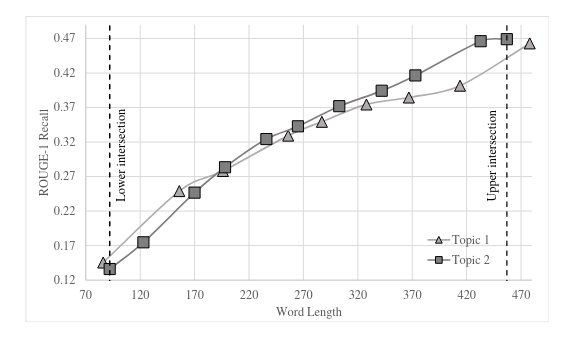
\includegraphics[height=8cm]{recall cureve.png}
     	\end{center}
     	\caption{ یک نمونه از نمودار منحنی بازیابی بر اساس طول \cite{shapira-etal-2021-extending}}
     	\label{fig:recall_curve}
     	\small{این نمودار دو تعامل متفاوت با سیستم خلاصه‌سازی را مقایسه می‌کند. هر نقطه نمایانگر   خروجی هر مرحله تعامل با کاربر است.}
     	\medskip
     	
     \end{figure}
     
     
     
  
   شاپیرا و همکاران برای بهبود مدل اینت‌سام و بهبود سرعت عمل در پاسخ‌گویی، توانایی پردازش کامل متون طولانی و رعایت تعادل میان اطلاعات کلی مقاله و اطلاعات مورد نیاز کاربر یک مدل جدید ارائه داده‌‌اند.
 ورودی این مدل  مجموعه‌ی اسناد، کوئری و تاریخچه‌ی تعاملات با کاربر به همراه خروجی‌ قبلی است.
 در ابتدا تعبیه کوئری به تعبیه اسناد ورودی الحاق شده  سپس امتیاز $ qMMR $ با استفاده از مدل $ RL-MMR $ ‌محاسبه می‌شود. هدف این امتیاز  ایجاد خلاصه‌ای شبیه به اسناد ورودی و کوئری و متفاوت از تاریخچه است.
 سپس با استفاده از مکانیزم توجه با مرکزیت دوگانه
  \LTRfootnote{two hub attention}
  بر اساس کدگذاری به دست آمده از تاریخچه و مدل $ RL-MMR $ ‌

 توزیع احتمال هر جمله را به دست ‌می‌آید.
مدل ام‌سام
\LTRfootnote{MSumm}
 یک مدل خودرگرسیون
 \LTRfootnote{Autoregressive}
است  که برای آموزش آن از یادگیری تقویتی به همراه مکانیسم پاداش دوگانه استفاده می‌شود.   معیار دلتا-روژ 
  \LTRfootnote{Delta-ROUGE}
  برای سنجش میزان اطلاعات اضافه‌ی خروجی نسبت به خروجی‌های قبلی و شباهت واژگانی و معنایی  برای سنجش میزان شباهت خروجی به کوئری به عنوان پاداش استفاده شده‌اند.
    مدل $ RL-MMR $ ‌ موجب افزایش سرعت پردازش اطلاعات در مدل و پردازش کامل مجموعه‌ی اسناد و مکانیزیم پاداش دوگانه  تعادل موجب ایجاد تعادل اطلاعات می‌شود.    ساختار مدل در شکل  \ref{fig:MSumm}  نشان داده شده است
    \cite{shapira-etal-2022-interactive}.
% برای پردازش سریع و کامل متون از مدل $ RL-MMR $ ‌و برای رعایت تعادل از یک مکانیسم پاداش دوگانه  (میزان شباهت خروجی به کوئری و میزان اطلاعات اضافه‌ی خروجی نسبت به خروجی‌های قبلی )استفاده شده است. 
  

    \begin{figure}[!h]
	\begin{center}
		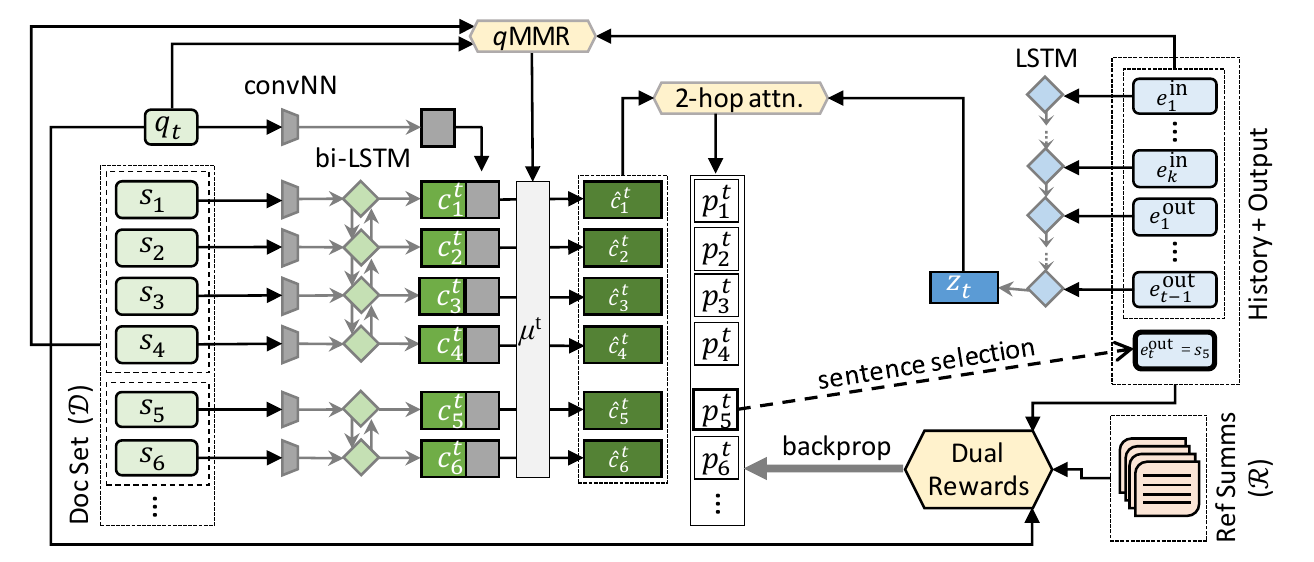
\includegraphics[height=7cm]{query-assited.png}
	\end{center}
	\caption{ معماری مدل  ام‌سام \cite{shapira-etal-2022-interactive}} 
	\label{fig:MSumm}
	
	\medskip
	
\end{figure}


	%  ایجاد معیارهای جدید ارزیابی براساس منابعی غیر از خلاصه‌های مبنایی2. معیار روژ   دارای سه محدودیت اصلی است: تعصب آن نسبت به شباهت واژگانی، توجه کم آن به روان بودن و خوانایی خلاصه‌های انتزاعی تولید شده ، و پیش نیاز سخت آن برای استفاده از خلاصه‌های حقیقت پایه برای تولید امتیازات. علاوه بر این، خلاصه‌های تولید شده با معیار روژ بالا معمولاً جذابیت انسانی پایینی دارند ، بنابراین، محققان معیارهای جدیدی را برای افزایش تازگی [16]، سازگاری واقعی[17] و کیفیت بر اساس پاسخ به پرسش و رتبه‌بندی انسانی [17] با استفاده از رویکردهای پاداش‌دهی یادگیری تقویتی بدون نیاز به خلاصه‌های مبنایی ایجاد کردند.




%استفاده از برآورد درست‌نمایی بیشینه  در مدل‌های خلاصه‌سازی  ممکن است  با. به همین دلیل، یادگیری تقویتی به عنوان جایگزینی برای بهینه‌سازی مستقیم مدل‌ها بر روی معیارهای ارزیابی و پاداش صریح به کیفیت پیش‌بینی‌های مدل استفاده شده است. 
